\documentclass{standalone}

\usepackage{amssymb}
\usepackage{tikz}
\usetikzlibrary{calc}
\usetikzlibrary{decorations}
\usetikzlibrary{decorations.markings}

\begin{document}
  %noformat{
  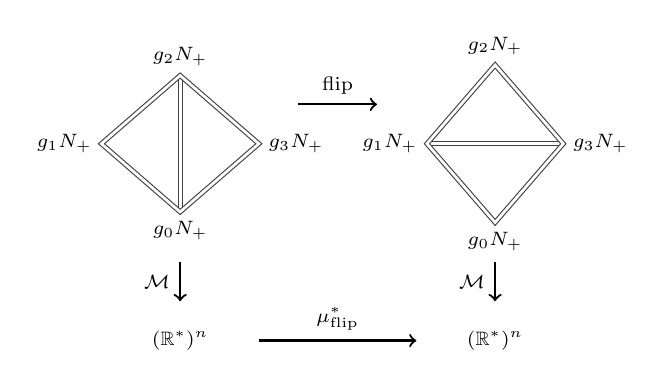
\begin{tikzpicture}
    \tikzstyle{te} = [color=darkgray, double distance=1pt]

    \tikzset{font=\scriptsize}

    \begin{scope}[shift={(0.0,0.0)}]
      \coordinate[label=270:{$g_0N_{+}$}] (v0) at ($ (300:1.0) + (180:0.5) $);
      \coordinate[label=180:{$g_1N_{+}$}] (v1) at ($ (180:0.5) + (180:0.5) $);
      \coordinate[label= 90:{$g_2N_{+}$}] (v2) at ($ ( 60:1.0) + (180:0.5) $);

      \coordinate[label=  0:{$g_3N_{+}$}] (v3) at ($ (  0:0.5) + (  0:0.5) $);

      \draw[te] (v0) to (v2);
      \draw[te] (v0) to (v1) to (v2) to (v3) to cycle;
    \end{scope}

    \begin{scope}[shift={(4.0,0.0)}]
      \coordinate[label=180:{$g_1N_{+}$}] (v1) at ($ (210:1.0) + ( 90:0.5) $);
      \coordinate[label= 90:{$g_2N_{+}$}] (v2) at ($ ( 90:0.5) + ( 90:0.5) $);
      \coordinate[label=  0:{$g_3N_{+}$}] (v3) at ($ (330:1.0) + ( 90:0.5) $);

      \coordinate[label=270:{$g_0N_{+}$}] (v0) at ($ (270:0.5) + (270:0.5) $);

      \draw[te] (v1) to (v3);
      \draw[te] (v0) to (v1) to (v2) to (v3) to cycle;
    \end{scope}

    \node (c1) at (0.0, -2.5) {$(\mathbb{R}^{\ast})^n$};
    \node (c2) at (4.0, -2.5) {$(\mathbb{R}^{\ast})^n$};

    \draw[->, thick]
        (1.5,0.5)
        to[] node[midway, above] (t06) {$\mathrm{flip}$}
        (2.5,0.5);
    \draw[->, thick]
        (0.0,-1.5)
        tonode[midway, left] (t01) {$\mathcal{M}$}
        (0.0,-2.0);
    \draw[->, thick]
        (4.0,-1.5)
        tonode[midway, left] (t02) {$\mathcal{M}$}
        (4.0,-2.0);
    \draw[->, thick]
        (1.0,-2.5)
        to[] node[midway, above] (t05) {$\mu_{\mathrm{flip}}^{\ast}$}
        (3.0,-2.5);
  \end{tikzpicture}
  %}noformat
\end{document}
